
%\marginlabel{\bf {\tt .rea} files:}
The {\tt .rea} file consists of several sections. The mesh specifications  with {\bf geometry}, {\bf curvature} and {\bf boundary conditions} are in the second section.

\subsubsection*{ Parameters and logical switches}
\begin{description}
\item{\bf parameters} These control the runtime parameters such as viscosity,
    conductivity, number of steps, timestep size, order of the timestepping,
    frequency of output, iteration tolerances, flow rate, filter strength,
    etc.   There are also a number of free parameters that the user can
    use as handles to be passed into the user defined routines in the .usr file.
\item{\bf passive scalar data} This information can be specified also in the \texttt{.uservp} routine in the .usr file. If specified in the .rea file then the coefficients for the conductivity term are listed in ascending order for passive scalars ranging \texttt{1..9} followed by the values for the \(\rho c_p\) coefficients.
\begin{verbatim}
4  Lines of passive scalar data follows 2 CONDUCT; 2 RHOCP
   1.00000       1.00000       1.00000       1.00000       1.00000
   1.00000       1.00000       1.00000       1.00000
   1.00000       1.00000       1.00000       1.00000       1.00000
   1.00000       1.00000       1.00000       1.00000
\end{verbatim}
\item{\bf logicals} These determine whether one is computing a steady or unsteady
  solution, whether advection is turned on, etc.
\end{description}

Next we have the logical switches as follow, a detailed explanation to be found in Sec:\ref{sec:switches}
\begin{verbatim}
           13  LOGICAL SWITCHES FOLLOW
  T     IFFLOW
  T     IFHEAT
  T     IFTRAN
  T T F F F F F F F F F IFNAV & IFADVC (convection in P.S. fields)
  F F T T T T T T T T T T IFTMSH (IF mesh for this field is T mesh)
  F     IFAXIS
  F     IFSTRS
  F     IFSPLIT
  F     IFMGRID
  F     IFMODEL
  F     IFKEPS
  F     IFMVBD
  F     IFCHAR
\end{verbatim}
\subsubsection*{Mesh and boundary condition info} 
\begin{description}
\item{\bf geometry} The geometry is specified in an arcane format specifying
    the \(xyz\) locations of each of the eight points for each element,
    or the \(xy\) locations of each of the four points for each element in 2D.
A line of the following type may be encountered at the beginning of the mesh section of the area file.    
\begin{verbatim}
3.33333       3.33333     -0.833333      -1.16667     XFAC,YFAC,XZERO,YZERO
\end{verbatim}
This part is to be read by Prenek and provides the origin of the system of coordinates \texttt{XZERO;YZERO} as well as the size of the cartesian units \texttt{XFAC;YFAC}. This one line has no impact on the mesh as being read in Nek5000. 

The header of the mesh data may have the following representation
\begin{center}
\begin{verbatim} **MESH DATA** 6 lines are X,Y,Z;X,Y,Z. Columns corners 1-4;5-8
      226  3         192           NEL,NDIM,NELV
    
\end{verbatim}
\end{center}
The header states first how many elements are available in total (\(226\)), what dimension is the the problem (here three dimensional), and how many elements are in the fluid mesh (\(192\)). 
Following the header, all elements are listed. The fluid elements are listed first, followed by all solid elements if present. In this case there are (\(34\)) solid elements.

The data following the header is formatted as shown in Table.~\ref{tab:element}. This provides all the coordinates of an element for top and bottom faces. The numbering of the vertices is shown in Fig.~\ref{fig:elorder}. The header for each element as in Table.~\ref{tab:element}, i.e. \texttt{[1A] GROUP} is reminiscent of older Nek5000 format and does not impact the mesh generation at this stage.\footnote{we are inquiring whether other groups still use it}

%\begin{center}
%     \begin{tabular}{l|l|l|l}
%  0.000000E+00 & 0.171820E+00 & 0.146403E+00 & 0.000000E+00 \\
%  0.190000E+00 & 0.168202E+00 & 0.343640E+00 & 0.380000E+00 \\
%  0.000000E+00 & 0.000000E+00 & 0.000000E+00 & 0.000000E+00 \\
%  0.000000E+00 & 0.171820E+00 & 0.146403E+00 & 0.000000E+00 \\
%  0.190000E+00 & 0.168202E+00 & 0.343640E+00 & 0.380000E+00  \\
%  0.250000E+00 & 0.250000E+00 & 0.250000E+00 & 0.250000E+00  \\
%  \end{tabular}
%\end{center}

\begin{table}
\begin{center}
 \texttt{ELEMENT           1 [    1A]    GROUP    0}
\subfloat{
\begin{tabular}{l c c c c}
%\fontsize 
  \(\texttt{Face \{1,2,3,4\}}\)&&&&\\
  \(x_{1,\ldots,4}=\)& 0.000000E+00 & 0.171820E+00 & 0.146403E+00 & 0.000000E+00 \\
  \(y_{1,\ldots,4}=\)&0.190000E+00 & 0.168202E+00 & 0.343640E+00 & 0.380000E+00 \\
  \(z_{1,\ldots,4}=\)&0.000000E+00 & 0.000000E+00 & 0.000000E+00 & 0.000000E+00 \\
  \(\texttt{Face \{5,6,7,8\}}\)&&&&\\
  \(x_{5,\ldots,8}=\)&0.000000E+00 & 0.171820E+00 & 0.146403E+00 & 0.000000E+00 \\
  \(y_{5,\ldots,8}=\)&0.190000E+00 & 0.168202E+00 & 0.343640E+00 & 0.380000E+00  \\
  \(z_{5,\ldots,8}=\)&0.250000E+00 & 0.250000E+00 & 0.250000E+00 & 0.250000E+00  
  \end{tabular}} 
%\subfloat[Element]{\raisebox{-10pt}{\vspace{0.5cm}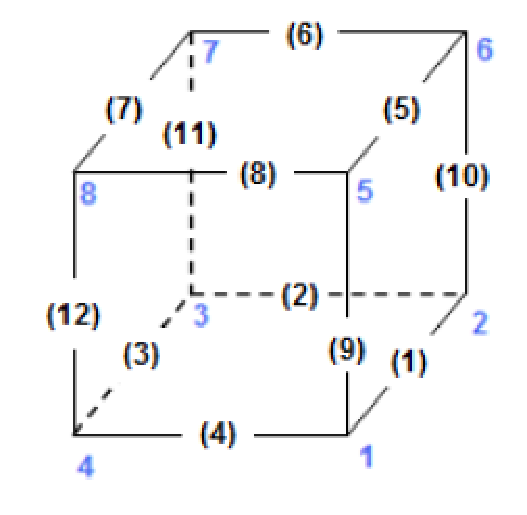
\includegraphics[scale=0.4]{3dcube}\label{fig:3dcube}}}
%{\begin{minipage}[c][1\width]{0.4\textwidth}\centering 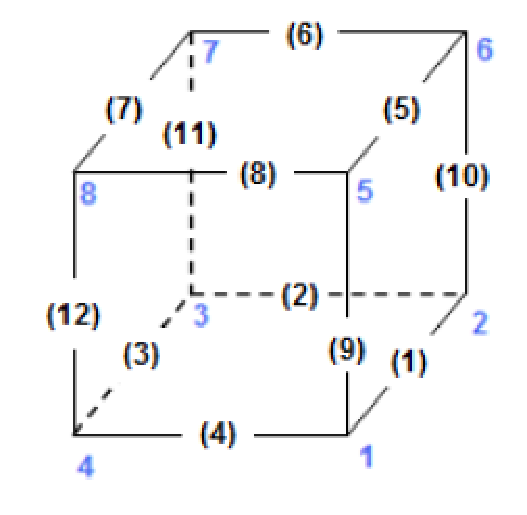
\includegraphics[width=0.4\textwidth]{3dcube} \end{minipage}}
\caption{Geometry description in .rea file}
\label{tab:element}
\end{center}
\end{table} 
\normalsize

\begin{figure}
\begin{center}
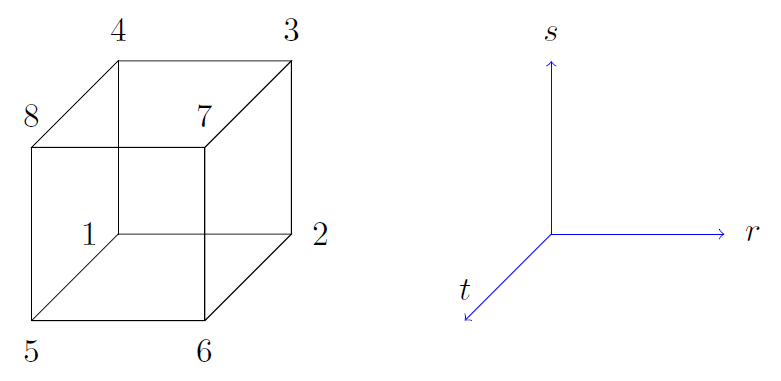
\includegraphics[scale=0.5]{3dcube_1.png}
\caption{Geometry description in .rea file (sketch of one element ordering - Preprocessor corner notation)}
\label{fig:elorder}
\end{center}
\end{figure}

\begin{figure}
\begin{center}
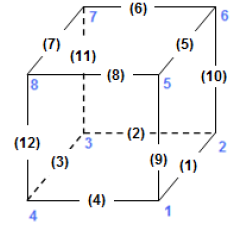
\includegraphics[scale=0.5]{3dcube.png}
\caption{Edge numbering in .rea file, the edge number is in between parenthesis. The other numbers represent vertices.}
\label{fig:edges}
\end{center}
\end{figure}

%(3,1) node[circle,draw](y) {$\int_1^2 x \mathrm d x$};
%\draw[->,blue] (x) -- (y);
%\draw[->,red] (x) -| node[near start,below] {label} (y);
%\draw[->,orange] (x) .. controls +(up:1cm) and +(left:1cm) .. 

%   Preprocessor Corner notation:    
%
%           4+-----+3    ^ s               
%           /     /|     |            
%          /     / |     |                     
%        8+-----+7 +2    +----> r       
%         |     | /     /                  
%         |     |/     /                    
%5        5+-----+6    t                    


\item{\bf curvature} 
     This section describes the curvature of the elements. It is expressed as deformation of the linear elements.  
     Therefore, if no elements are curved (if only linear elements are present) the section remains empty.

     The section header may look like this:

     \begin{center}
     \texttt{640 Curved sides follow IEDGE,IEL,CURVE(I),I=1,5, CCURVE}
     \end{center}

     Curvature information is provided by edge and element. Therefore up to 12 curvature entries can be present for each element.
Only non-trivial curvature data needs to be provided, i.e., edges that correspond to linear elements, since they have no curvature, will have no entry.
The formatting for the curvature data is provided in Table.~\ref{tab:midside}. 

\footnotesize
\begin{table} 
     \begin{center}
\begin{tabular}{ l|l|l|l|l|l|l|l }
   \hline
 \texttt{IEDGE}& \texttt{IEL} &\texttt{CURVE(1)} &\texttt{CURVE(2)}&\texttt{CURVE(3)}&\texttt{CURVE(4)}&\texttt{CURVE(5)}&\texttt{CCURVE} \\ \hline \hline
 9   &  2 & 0.125713  &   -0.992067 &      0.00000  &     0.00000 &      0.00000  &   m \\
10   & 38 & 0.125713 &    -0.992067  &     3.00000 &      0.00000  &     0.00000 &    m \\
 1   & 40 & 1.00000  &     0.000000  &     0.00000 &      0.00000  &     0.00000 &    C \\
   \hline
\end{tabular}  
\caption{Curvature information specification } 
\label{tab:midside}
\end{center}
\end{table}
\normalsize

     There are several types of possible curvature information represented by \texttt{CCURVE}. This include:
     \begin{itemize}
     \item 'C' stands for circle and is given by the radius of the circle,  in \texttt{CURVE(1)}, all other compoentns of the \texttt{CURVE} array are not used but need to be present. 
     \item 's' stands for sphere and is given by the radius and the center of the sphere, thus filling the first 4 components of the \texttt{CURVE} array. The fifth component needs to be present but is not utilized. 
     \item 'm' is given by the coordinates of the midside-node, thus using the first 3 components of the \texttt{CURVE} array, and leads to a second order reconstruction of the face.  The fourth and fifth components need to be present but are not utilized.
     \end{itemize}

Both 'C' and 's' types allow for a surface of as high order as the polynomial used in the spectral method, since they have an underlying analytical description, any circle arc can be fully determined by the radius and end points. However for the 'm' curved element descriptor the surface can be reconstructed only up to second order. This can be later updated to match the high-order polynomial after the GLL points have been distributed across the boundaries. This is the only general mean to describe curvature currrently in Nek5000 and corresponds to a HEX20 representation.

For better understanding let us focus on what the data in Table.~\ref{tab:midside} signifies. Edge $9$ of element $2$ has a edge  midpoint at $(0.125713, -0.992067, 0.00000)$  and so on. For edge numbering the reader is advised to check Fig.~\ref{fig:edges}, which illustrates the relationship between vertex numbering and edge numbering.

To maninpulate the geometry in Nek5000 at runtime, it is possible to use  usrdat2. In this subroutine the user can deform the geometry to match the intended surface, followed by a call to the subroutine 'fixgeom' which can realign the point distribution in the interior of the element.

We also note, that, unlike the geometry data, each curvature entry (as shown in Table.~\ref{tab:midside}) is formatted and the format is {\bf dependent on the total number of elements}. Three cases exist as shown in the code below: 
\footnotesize
\begin{verbatim}
                     if (nelgt.lt.1000) then
                        write(10,'(i3,i3,5g14.6,1x,a1)') i,eg,
     $                  (vcurve(k,i,kb),k=1,5),cc
                     elseif (nelgt.lt.1000000) then
                        write(10,'(i2,i6,5g14.6,1x,a1)') i,eg,
     $                  (vcurve(k,i,kb),k=1,5),cc
                     else
                        write(10,'(i2,i12,5g14.6,1x,a1)') i,eg,
     $                  (vcurve(k,i,kb),k=1,5),cc
\end{verbatim}
\normalsize
The fortran format is as follows:
\begin{itemize}
\item For a total number of elements below $1,000$ the format is \texttt{(i3,i3,5g14.6,1x,a1)}.
\item For a total number of elements $1,000$ - $999,999$ the format is \texttt{(i2,i6,5g14.6,1x,a1)}.
\item For a total number of elements above $999,999$ the format is \texttt{(i2,i12,5g14.6,1x,a1)}.
\end{itemize}


\begin{figure}
\begin{center}
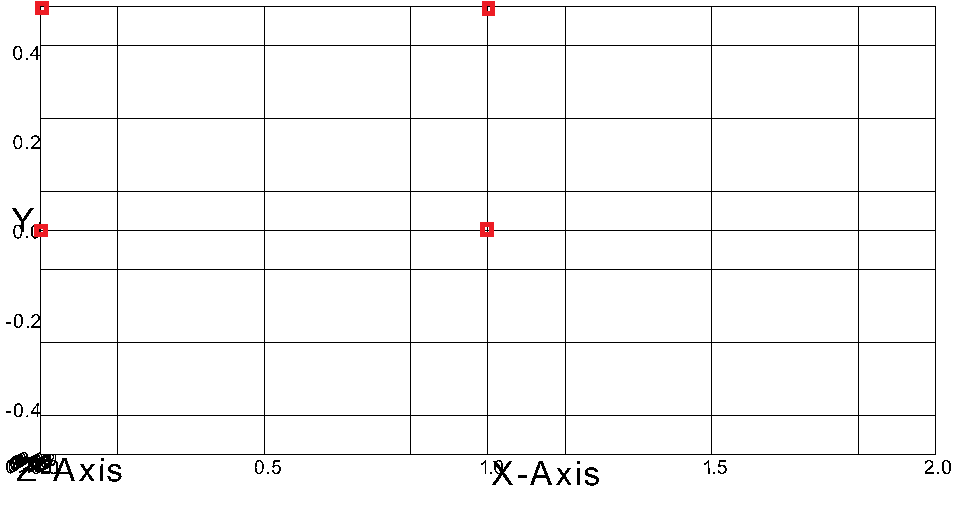
\includegraphics[scale=0.5]{base1.png}
\caption{Example mesh - without curvature. Square dots represent example vertices.}
\label{fig:ex1}
\end{center}
\end{figure}

\begin{figure}
\begin{center}
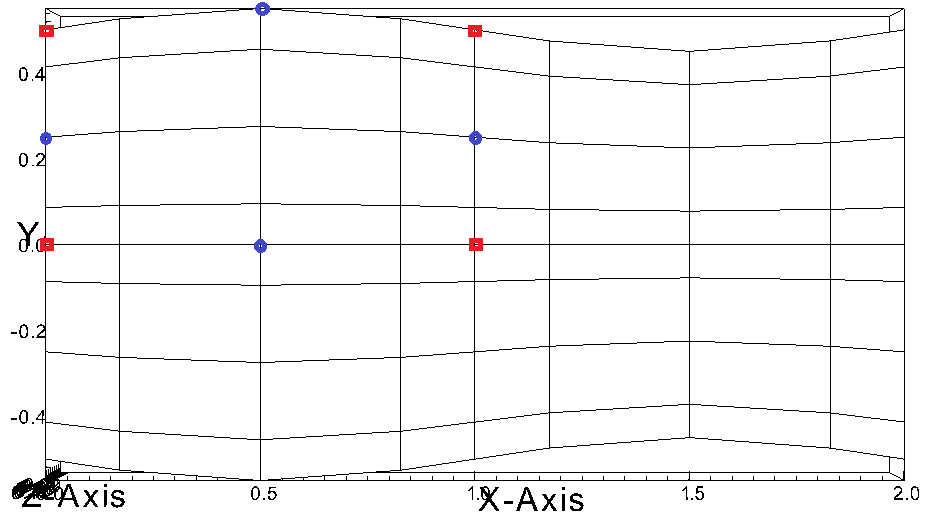
\includegraphics[scale=0.5]{modified1.png}
\caption{Example mesh -  with curvature. Circular dots represent example midsize points. }
\label{fig:ex2}
\end{center}
\end{figure}


To further illustrate the usage of curvature data, let us examine an example of .rea file with and wiuthout curvature information and the corresponding mesh representation. Figure~\ref{fig:ex1} represents a 12 element box mesh (2x2x3, with periodic conditions in z) without curvature, while Fig.~\ref{fig:ex2} presents the same mesh with a sinusoidal deformation in direction y. Only two edges per element are curved. 
The input for the mesh without curvature is:

\input mesh_example

The input for the mesh with curvature is: 

\input mesh_curv_example

Note that element and boundary condition information are identical between the two cases.

\item{\bf boundary conditions} 
     Boundary conditions (BCs) are specified for each field in sequence: velocity, temperature and passive scalars. The section header for each field will be as follows (example for the velocity):
     \begin{center}
     \texttt{ ***** FLUID   BOUNDARY CONDITIONS *****}

     \end{center}
     and the data is stored as illustarted in Table.~\ref{tab:bcs}. For each field boundary conditions are listed for each face of each element. 

Boundary conditions are given in order per each element, see Table.~\ref{tab:bcs} column \texttt{IEL}, and faces listed in ascending order $1-6$ in column \texttt{IFACE}. Note that the header in Table.~\ref{tab:bcs} does not appear in the actual \texttt{.rea}.
The ordering for faces each element is shown in Fig.~\ref{fig:forder}. A total equivalent to $6N_{field}$ boundary conditions are listed for each field, where $N_{field}$ is the number of elements for the specific field. $N_{field}$ is equal to the total number of fluid elements for the velocity and equal to the total number of elements (including solid elements) for temperature. For the passive scalars it will depend on the specific choice, but typically scalars are solved on the temeprature mesh (solid+fluid). 

\begin{figure}
\begin{center}
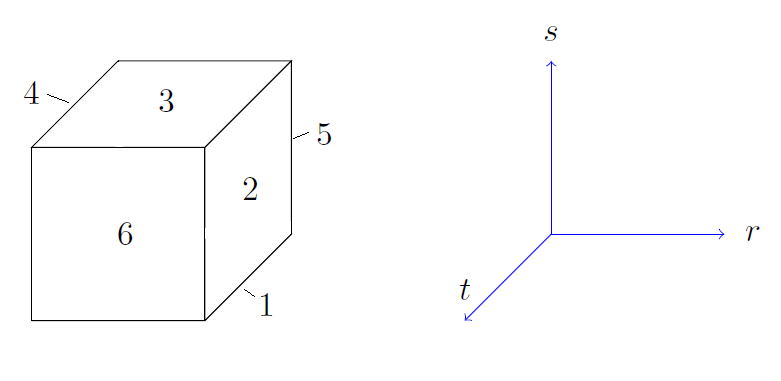
\includegraphics[scale=0.5]{3dcube_2.png}
\caption{Face ordering for each element.}
\label{fig:forder}
\end{center}
\end{figure}

Each BC letter condition is formed by three characters. Common BCs include:
\begin{enumerate}
\item {\tt E} - internal boundary condition. No additional information needs to be provided.
\item {\tt SYM} - symmetry boundary condition. No additional information needs to be provided.
\item {\tt P} - periodic boundary conditions,  which indicates that an element face is connected to another element to establish a periodic BC. The connecting element and face need be  to specified in {\tt CONN-IEL} and {\tt CONN-IFACE}. 
\item {\tt v} - imposed velocity boundary conditions (inlet). The value is specified in the user subroutines. No additional information needs to be provided in the .rea file.
\item {\tt W} - wall boundary condition (no-slip) for the velocity. No additional information needs to be provided.
\item {\tt O} - outlet boundary condition (velocity). No additional information needs to be provided.
\item {\tt t} - imposed temperature  boundary conditions (inlet). The value is specified in the user subroutines. No additional information needs to be provided in the .rea file.
\item {\tt f} - imposed heat flux  boundary conditions (temperature). The value is specified in the user subroutines. No additional information needs to be provided in the .rea file.
\item {\tt I} - adiabatic boundary conditions (temeperature). No additional information needs to be provided.
\end{enumerate}

Many of the BCs support either a constant specification or a user defined specification which may be an arbitrary function.   For example, a constant Dirichlet BC for velocity is specified by {\tt V}, while a user defined BC is specified by {\tt v}.   This upper/lower-case distinction is  used for all cases.   There are about 70 different types of boundary conditions in all, including free-surface, moving boundary, heat flux, convective cooling, etc. The above cases are just the most used types.
    
\footnotesize 
\begin{table}  
\begin{center}
\begin{tabular}{ l|l|l|l|l|l|l|l }
   \hline
 \texttt{CBC}& \texttt{IEL} &\texttt{IFACE} &\texttt{CONN-IEL}&\texttt{CONN-IFACE} &  &  & \\ \hline \hline
  E   & 1 & 1 &  4.00000   &    3.00000  &     0.00000      &     0.00000 &     0.00000 \\
   ..   & .. & .. &  ..   &   .. &    ..   &   .. &    ..   \\
   W  &  5 & 3 &  0.00000  &     0.00000  &     0.00000   &     0.00000 &     0.00000  \\
    ..   & .. & .. & ..   &   ..  &    ..   &   .. &    ..   \\
   P  &  23 & 5  & 149.000 &      6.00000  &     0.00000 &     0.00000 &     0.00000  \\
   \hline
\end{tabular} 
\caption{Formatting of boundary conditions input.}
\label{tab:bcs}  
\end{center}
\end{table}
\normalsize

As in the case of the curvature entries, the boundary conditions entries are formatted and {\bf the format is dependent on the total number of elements}.  
The code below shows an example of writing statement for boundary conditions:

\footnotesize
\begin{verbatim}
                  if (nlg.lt.1000) then
                     write(10,'(a1,a3,2i3,5g14.6)')
     $               chtemp,s3,eg,i,(vbc(ii,i,kb),ii=1,5)
                  elseif (nlg.lt.100000) then
                     write(10,'(a1,a3,i5,i1,5g14.6)')
     $               chtemp,s3,eg,i,(vbc(ii,i,kb),ii=1,5)
                  elseif (nlg.lt.1000000) then
                     write(10,'(a1,a3,i6,5g14.6)')
     $               chtemp,s3,eg,(vbc(ii,i,kb),ii=1,5)
                  else
                     write(10,'(a1,a3,i12,5g18.11)')
     $               chtemp,s3,eg,(vbc(ii,i,kb),ii=1,5)
                  endif
\end{verbatim}
\normalsize

The fortran format is as follows:
\begin{itemize}
\item For a total number of elements below $1,000$ the format is \texttt{(a1,a3,2i3,5g14.6)}.
\item For a total number of elements $1,000$ - $99,999$ the format is \texttt{(a1,a3,i5,i1,5g14.6)}.
\item For a total number of elements $100,000$ - $999,999$ the format is \texttt{(a1,a3,i6,5g14.6)}.
\item For a total number of elements above $999,999$ the format is \texttt{(a1,a3,i12,5g18.11)}.
\end{itemize}
We note that:
\begin{itemize}
\item The first item in the format for each of the four cases is a string containing a space.
\item The second item in the format for each of the four cases is a string specifying the boundary condition type.
\item In cases where the total number of elements is bigger than 99,999, the \texttt{IFACE} item is omitted. Given that Nek5000 already knows the ordering of the actual faces within each element in column \texttt{IFACE} is in fact not needed.
\item The number of significant digits increases in the fourth case. This is needed for periodic boundary conditions.
\end{itemize}
     
\end{description}

\subsubsection*{ Output info} 
\begin{description}
\item{\bf restart conditions} 

     Here, one can specify a file to use as an initial condition.
     The initial condition need not be of the same polynomial order
     as the current simulation.   One can also specify that, for example,
     the velocity is to come from one file and the temperature from another.
     The initial time is taken from the last specified restart file, but 
     this can be overridden.
\item{\bf history points}

The following section defines history points in the {\tt .rea} file, see example {\tt vortex/r1854a.rea}, or {\tt shear4/shear4.rea}
\begin{verbatim}
0 PACKETS OF DATA FOLLOW
***** HISTORY AND INTEGRAL DATA *****
    56 POINTS. H code, I,J,H,IEL 
UVWP    H     31     31   1   6
UVWP    H     31     31   31  6
UVWP    H     31     31   31  54
 "      "      "      "    "   "
\end{verbatim}

The {\tt "56 POINTS"} line needs to be followed by 56 lines of the type shown. However, in each of the following lines, which have the {\tt UVWP} etc., location is CRUCIAL, it
must be layed out exactly as indicated above\footnote{these lines contain character strings, they use formatted reads}, it is therefore advisable to refer to the examples {\tt vortex, shear4}.  If you want to pick points close to the center of element 1 and are running with lx1=10, say, you might choose {\tt UVWP H 5 5 5 1}. \footnote{the indicated point would really be at the middle of the element only if lx1=9}

The UVWP tells the code to write the 3 velocity components and pressure to the .sch file at
each timestep (or, more precisely, whenever {\tt mod(istep,iohis)=0}, where {\tt iohis=param(52))}.
Note that if you have more than one history point then they are written sequentially at each
timestep. Thus 10 steps in the first example with {\tt param(52)=2} would write {\tt (10/2)*56 = 280}
lines to the .sch file, with 4 entries per line. The "H" indicates that the entry corresponds to a requested history point. A note of caution: if the {\tt ijk} values (5 5 5 in the preceding example line) exceed {\tt lx1,ly1,lz1} of your SIZE file, then they are truncated to that value. For example, if {\tt lx1=10} for the data at the top (31 31 31) then the code will use {\tt ijk} of (10 10 10), plus the given element number, in identifying the history point. It is often useful to set {\tt ijk} to large values (i.e., > {\tt lx1}) because the endpoints of the spectral element mesh are invariant when {\tt lx1} is changed. 

\begin{comment}
A difficulty with the current nek history point specification is finding the requisite ijke (e=element
number) values that correlate to the point of interest. There is a way to do this in postx that
is relatively painless, but this is not useful for very large problems. (The approach is:
SET PLOT FORMAT
SCALAR
VALUES
PLOT
Follow the instructions and for each point requested, postx will write to the screen lines that
are similar to the above, ready to be pasted into the .rea file.)
8. When you run nek, it will write the coordinate information to the logfile on the first timestep
so that you can verify the point locations.
\end{comment}
\item{\bf output specifications} 
     Outputs are discussed in a separate section of the manual, available online.
\end{description}


\noindent
It is important to note that Nek5000 currently supports two input file
formats, ASCII and binary.   The {\tt .rea} file format
described above is ASCII.  For the binary format, all sections
of the .rea file having storage requirements that scale with 
number of elements (i.e., geometry, curvature, and boundary 
conditions) are moved to a second, {\tt .re2}, file and
written in binary.   The remaining sections continue to 
reside in the {\tt .rea} file.   The distinction between
the ASCII and binary formats is indicated in the {\tt .rea}
file by having a negative number of elements.
There are converters, {\tt reatore2} and {\tt re2torea}, in the Nek5000
tools directory to change between formats.   The binary file
format is the default and important for {\tt I/O} performance when the
number of elements is large ( \(>\) 100000, say).
